
\chapter{图像超分辨率算法定义} 

单幅图像超分辨率算法是一种利用一幅经过下采样、反卷积等“退化”过程后的低分辨率图像经过一系列的计算方法得到对应高分辨率图像的计算过程,图像退化计算可以建模为:
\begin{equation}
    \label{eq:example}
    I_L = D \left( I_H ; \mu  \right)
\end{equation}

\begin{figure}[h]
    \centering
    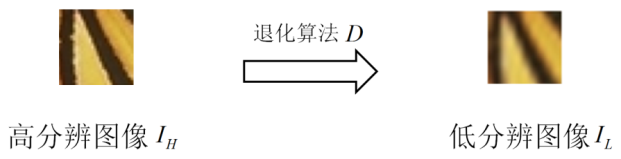
\includegraphics[width=0.42\linewidth]{./content/test.png}
    \caption{示例图片}
    \label{fig:example}
\end{figure}

图像超分辨率计算过程可建模如\eqref{eq:example}

\begin{figure}[h]
    \centering
    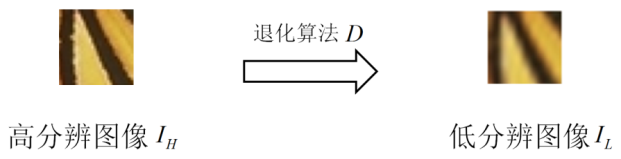
\includegraphics[width=0.42\linewidth]{./content/test.png}
    \caption{示例图片2}
    \label{fig:example2}
\end{figure}

\begin{figure}[h]
    \centering
    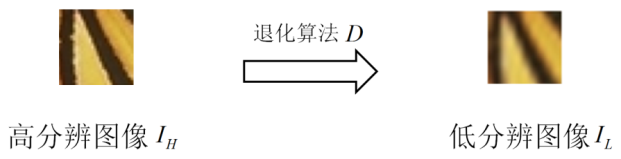
\includegraphics[width=0.42\linewidth]{./content/test.png}
    \caption{示例图片3}
    \label{fig:example3}
\end{figure}


其中,$I_L$为低分辨率图像,$I_H$为与之对应的高分辨图像,$D$代表一种图像退化算法,$\mu$为退化因子, 为经超分算法得到的高分辨率图像,$S$代表一种超分辨率算法,$v$为超分因子。

\section{超分辨率重建与生成对抗策略}

生成对抗策略是近几年来深度学习领域研究者重点研究方向。通过生成模型与判别器模型的对抗实现从输入源数据自身概率分布道目标数据的概率分布之间的函数映射参数的获取,从而获得一个源数据到目标数据的映射参数网络,这样相互迭代式的无监督学习方法提高了网络学习效率。…………。经典的生成对抗网络模型如下表示[26]:

生成对抗策略是近几年来深度学习领域研究者重点研究方向。通过生成模型与判别器模型的对抗实现从输入源数据自身概率分布道目标数据的概率分布之间的函数映射参数的获取,从而获得一个源数据到目标数据的映射参数网络,这样相互迭代式的无监督学习方法提高了网络学习效率。…………。经典的生成对抗网络模型如下表示[26]:
\begin{equation}
    \int f(x) \dif x
\end{equation}

生成对抗策略是近几年来深度学习领域研究者重点研究方向。通过生成模型与判别器模型的对抗实现从输入源数据自身概率分布道目标数据的概率分布之间的函数映射参数的获取,从而获得一个源数据到目标数据的映射参数网络,这样相互迭代式的无监督学习方法提高了网络学习效率。…………。经典的生成对抗网络模型如下表示[26]:




\begin{table}[h]
    \centering
    \caption{数据库间内容对比 }
    \begin{tabular}{cccccc}
      \toprule
      数据库  & 原始图像数 & 失真图像数 & 失真类型 & 主观评价法 & 参评人员数 \\
      \midrule
      LIVE    & 29         & 779        & 5       & DMOS       & 161        \\
      TID2013 & 25         & 3000       & 24      & MOS        & 971        \\
      \bottomrule
    \end{tabular}
    \label{tab:three-line}
  \end{table}